\begin{frame}
\frametitle{Планирование потоков}
\begin{itemize}
  \item Мы знаем что-такое потоки и как между ними переключаться
  \begin{itemize}
    \item осталось разобраться с мелочами - когда и на какой конкретно поток
    переключаться.
  \end{itemize}
  \item Начнем с простой и нереалистичной задачи:
  \begin{itemize}
    \item мы заранее знаем все задачи, которые нужно выполнить;
    \item и про каждую задачу знаем сколько времени потребуется на выполнение;
    \item более того мы выполняем каждую задачу от начала до конца без
    переключений, т. е. нужно только определить порядок выполнения задач.
  \end{itemize}
\end{itemize}
\end{frame}

\begin{frame}
\frametitle{SJF 1/2}
\begin{columns}
  \begin{column}{0.5\linewidth}
    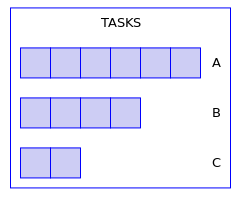
\includegraphics[width=0.9\linewidth]{sjf_tasks.png}
  \end{column}
  \begin{column}{0.5\linewidth}
    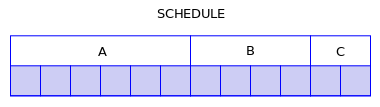
\includegraphics[width=0.9\linewidth]{sjf_schedule0.png}
    \begin{itemize}
      \item 3 задачи, по 6, 4 и 2 единиц;
      \item суммарно 12 единиц времени;
      \item среднее время ожидания заверешения:
      ${{6+10+12}\over{3}}=9.\left(3\right)$
    \end{itemize}
  \end{column}
\end{columns}
\end{frame}

\begin{frame}
\frametitle{SJF 2/2}
\begin{columns}
  \begin{column}{0.5\linewidth}
    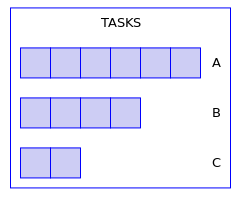
\includegraphics[width=0.9\linewidth]{sjf_tasks.png}
  \end{column}
  \begin{column}{0.5\linewidth}
    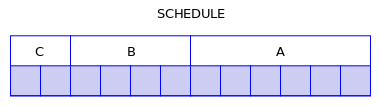
\includegraphics[width=0.9\linewidth]{sjf_schedule1.png}
    \begin{itemize}
      \item теже 3 задачи, по 6, 4 и 2 единиц;
      \item суммарно 12 единиц времени (о чудо!);
      \item среднее время ожидания заверешения:
      ${{2+6+12}\over{3}}=6.\left(6\right)$
    \end{itemize}
  \end{column}
\end{columns}
\end{frame}

\begin{frame}
\frametitle{Shortest Job First}
\begin{itemize}
  \item Упорядочив задачи по времени исполнения от меньшей к большей получим
  оптимальное по среднему времени ожидания расписание
  \begin{itemize}
    \item отсюда и Shortest Job First (SJF).
  \end{itemize}
\end{itemize}
\end{frame}

\begin{frame}
\frametitle{Блокировка потока}
\begin{itemize}
  \item Потоки могут быть заблокированы:
  \begin{itemize}
    \item поток может ожидать ввода от пользователя - даже самый быстрый
    пользователь очень медленный по сравнению с CPU;
    \item поток может ожидать получения данных по сети;
    \item поток может запросить доступ к медленному устройству и ждать
    прерывания от него (например, диск);
    \item другими словами поток может быть заблокирован в ожидании завершения
    операции ввода/вывода.
  \end{itemize}
  \item Заблокированным потокам нет смысла отдавать CPU:
  \begin{itemize}
    \item все что они могут делать, так это ждать завершения IO.
  \end{itemize}
\end{itemize}
\end{frame}

\begin{frame}
\frametitle{Динамическое создание и завершение}
\begin{itemize}
  \item Потоки создаются и завершаются динамически:
  \begin{itemize}
    \item новый поток может быть создан в любой момент;
    \item т. е. все потоки заранее не известны;
    \item существующий поток может завершиться;
    \item т. е. мы не знаем время необходимое потоку для завершения.
  \end{itemize}
\end{itemize}
\end{frame}

\begin{frame}
\frametitle{Round Robin}
\begin{itemize}
  \item Самый простой вариант планирования в реалистичных условиях - отдавать
  процессор активным потокам по очереди:
  \begin{itemize}
    \item все задачи ожидающие CPU организованы в очередь;
    \item каждой задаче выделяется квант времени;
    \item задача снимается с CPU по истечении кванта;
    \item задача может отдать CPU самостоятельно перед истечением кванта;
    \item незавершившаяся задача снятая с CPU возвращается в конец очереди.
  \end{itemize}
\end{itemize}
\end{frame}

\begin{frame}
\frametitle{Round Robin, pros}
\begin{itemize}
  \item Round Robin - является простым реалистичным алгоритмом планирования:
  \begin{itemize}
    \item выбор следующего потока требует $O\left(1\right)$;
    \item зная ограничение на количество потоков, мы можем ограничить
    максимальное время ожидания.
  \end{itemize}
  \item Гарантия, когда время реакции системы на событие (прерывание) жестко
  ограничено сверху - гарантия жесткого реального времени:
  \begin{itemize}
    \item т. е. Real Time на самом деле - это не про скорость;
    \item Round Robin сам по себе не нарушает гарантию реального времени.
  \end{itemize}
\end{itemize}
\end{frame}

\begin{frame}
\frametitle{Round Robin, cons 1/3}
\begin{itemize}
  \item IO Bounded поток - поток, работа которого ограничена скоростью IO:
  \begin{itemize}
    \item такие потоки часто не вырабатывают свой квант полностью, а отдают
    CPU раньше заблокировавшись на IO;
    \item типичный пример: текстовый редактор.
  \end{itemize}
  \item CPU Bounded поток - работа потока ограничивается скоростью CPU:
  \begin{itemize}
    \item такие потоки редко не вырабатывают свой квант полностью, они всегда
    хотят получить CPU в свое пользование;
    \item типичные примеры: численные расчеты, задачи рендеринга.
  \end{itemize}
\end{itemize}
\end{frame}

\begin{frame}
\frametitle{Round Robin, cons 2/3}
\begin{center}
  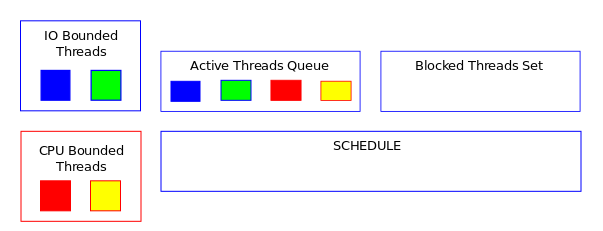
\includegraphics[width=0.8\linewidth]{rr0.png}
\end{center}
\begin{center}
  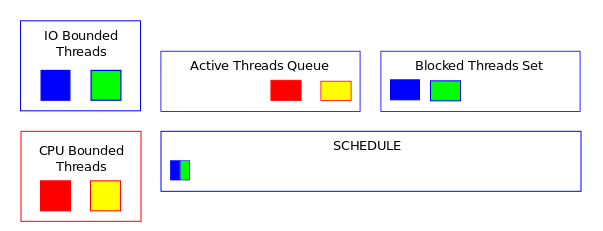
\includegraphics[width=0.8\linewidth]{rr1.png}
\end{center}
\end{frame}

\begin{frame}
\frametitle{Round Robin, cons 2/3}
\begin{center}
  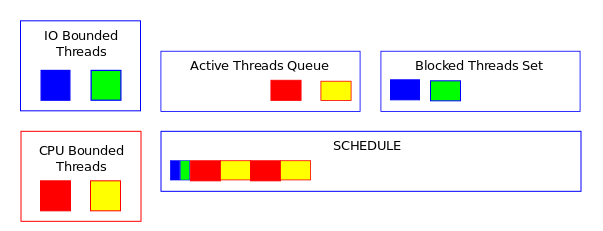
\includegraphics[width=0.8\linewidth]{rr2.png}
\end{center}
\begin{center}
  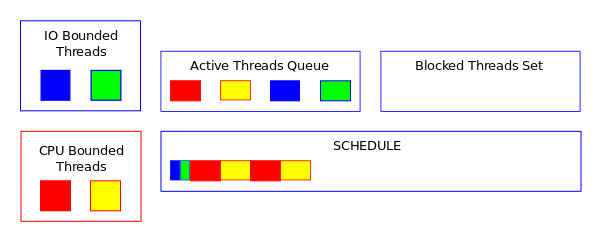
\includegraphics[width=0.8\linewidth]{rr3.png}
\end{center}
\end{frame}

\begin{frame}
\frametitle{Round Robin, cons 3/3}
\begin{center}
  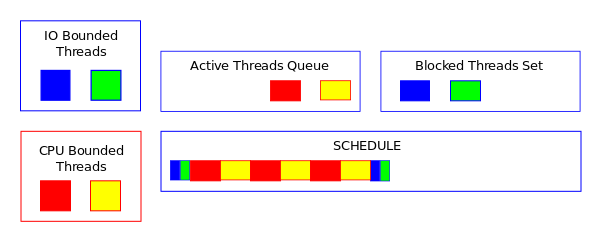
\includegraphics[width=0.8\linewidth]{rr4.png}
\end{center}
\begin{center}
  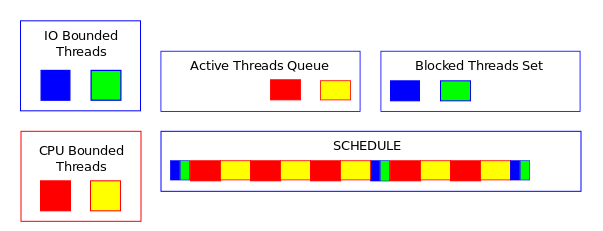
\includegraphics[width=0.8\linewidth]{rr5.png}
\end{center}
\end{frame}

\begin{frame}
\frametitle{Честность Round Robin}
\begin{itemize}
  \item IO Bounded задачи при Round Robin получают меньше CPU:
  \begin{itemize}
    \item они не вырабатывают свой квант и блокируются - не выработанное время
    никак не компенсируется.
  \end{itemize}
  \item IO Bounded задачи часто являются интерактивными, т. е. работают с
  пользователем, а пользователь не любит ждать
  \begin{itemize}
    \item однако когда поток разблокируется он встает в конец очереди и ждет
    пока вся очередь отработает.
  \end{itemize}
  \item Итого IO Bounded задачи получают меньше CPU, а задержка по доступу к CPU
  у них такая же как и у всех
  \begin{itemize}
    \item не все задачи одинаковые, и может потребоваться разделение задач на
    классы и приоритизация.
  \end{itemize}
\end{itemize}
\end{frame}

\begin{frame}
\frametitle{Completely Fair Scheduler 1/2}
\begin{itemize}
  \item Планировщик по-умолчанию в Linux Kernel
  \begin{itemize}
    \item пытается гарантировать идеальную честность отслеживая "виртуальное"
    отработанное время каждого потока;
    \item поток с нименьшим "виртуальным" временем получает CPU;
    \item выбор следующего потока требует $O\left(log n\right)$.
  \end{itemize}
\end{itemize}
\end{frame}

\begin{frame}
\frametitle{Completely Fair Scheduler 2/2}
\begin{itemize}
  \item Как обрабатывать разблокированные потоки вновь созданные потоки?
  \begin{itemize}
    \item нельзя просто верунть разблокированные задачи в очередь, т. к. их
    "виртуальное" время может сильно отстать от других и они станут "слишком
    приоритетными";
    \item для очереди потоков поддерживается "минимальное виртуальное" время,
    для новых и разблокированных задач проверяется, что их "виртуальное" время
    не сильно отстает от "минимального виртуального" времени.
  \end{itemize}
\end{itemize}
\end{frame}

\begin{frame}
\frametitle{Лотерейное планирование 1/2}
\begin{itemize}
  \item Самый "простой" способ обеспечить честность - рандомизация:
  \begin{itemize}
    \item выдадим каждому потоку набор лотерейных билетов;
    \item вероятность получения CPU в каждом "розыгыше" определяется количеством
    билетов у потока.
  \end{itemize}
  \item Статические и динамические приоритеты:
  \begin{itemize}
    \item потокам можно выдавать разное количество билетов согласно приоритету;
    \item кроме того, потоки могут временно передавать билеты друг другу и
    изменять свои приоритеты;
    \item например, поток \emph{A} пытается получить доступ к ресурсу \emph{X},
    но ресурс \emph{X} уже занят потоком \emph{B} - пусть \emph{A} передаст свои
    билеты \emph{B}, чтобы он раньше закончил работу с \emph{X}.
  \end{itemize}
\end{itemize}
\end{frame}

\begin{frame}
\frametitle{Лотерейное планирование 2/2}
\begin{itemize}
  \item При честной рандомизации возможны выбросы
  \begin{itemize}
    \item рандомизация гарантирует математическое ожидание времени CPU, но
    возможны отклонения от математического ожидания;
    \item чтобы ограничить отклонения, мы можем "удалять" выигравший билет;
    \item когда все билеты были "удалены", мы раздаем билеты заново;
    \item выбросы все еще возможны, но они ограничены (почти).
  \end{itemize}
\end{itemize}
\end{frame}
